\documentclass[tikz, border=5mm]{standalone}

\begin{document}

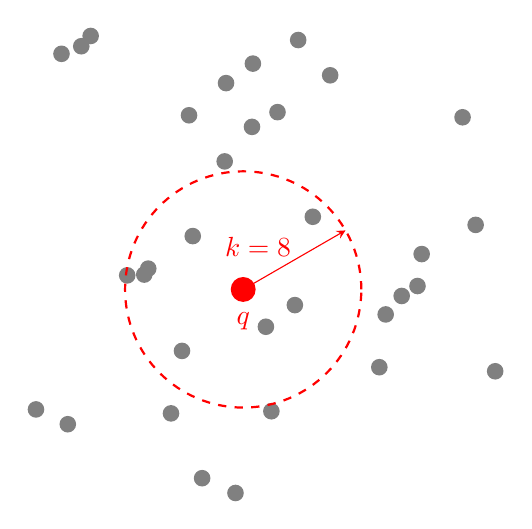
\begin{tikzpicture}[scale=6] % Escala ampliada para mejor visualización
    
    % Fijar la semilla para que la distribución uniforme sea reproducible
    \pgfmathsetseed{2026}

    % 1. Generar la nube de puntos uniformemente dispersos en el cuadrado [0,1]x[0,1]
    % 'rnd' genera un número pseudoaleatorio entre 0.0 y 1.0
    \foreach \i in {1,...,33} {
        \fill[gray] (rnd, rnd) circle (0.5pt);
    }

    % 2. Dibujar el cuadrado unitario
    %\draw[thick, black!50] (0,0) rectangle (1,1);
    
    % Etiquetas de los vértices (opcional, para dar contexto métrico)
    %\node[below left] at (0,0) {$(0,0)$};
    %\node[above right] at (1,1) {$(1,1)$};

    % 3. Definir y dibujar el punto de consulta (q)
    % Lo ubicamos de manera arbitraria pero representativa (ej. 0.45, 0.45)
    \coordinate (q) at (0.45, 0.45);
    \fill[red] (q) circle (0.75pt) node[below=5pt] {$q$};

    % 4. Dibujar el círculo centrado en q con radio 0.5
    % Se utiliza 'dashed' (punteado) para representar la frontera de vecindad
    \draw[red, thick, dashed] (q) circle (0.25);

    % 5. (Opcional) Dibujar un vector para indicar el radio exacto
    \draw[red, ->, >=stealth] (q) -- ++(30:0.25) node[midway, above left, inner sep=1pt] {$k=8$};

\end{tikzpicture}

\end{document}
